\documentclass{article}
\usepackage{physics}
\usepackage{graphicx}
\usepackage{caption}
\usepackage{amsmath}
\usepackage{bm}
\usepackage{framed}
\usepackage{authblk}
\usepackage{empheq}
\usepackage{amsfonts}
\usepackage{esint}
\usepackage[makeroom]{cancel}
\usepackage{dsfont}
\usepackage{centernot}
\usepackage{mathtools}
\usepackage{subcaption}
\usepackage{bigints}
\usepackage{amsthm}
\theoremstyle{definition}
\newtheorem{lemma}{Lemma}
\newtheorem{defn}{Definition}[section]
\newtheorem{prop}{Proposition}[section]
\newtheorem{rmk}{Remark}[section]
\newtheorem{thm}{Theorem}[section]
\newtheorem{exmp}{Example}[section]
\newtheorem{prob}{Problem}[section]
\newtheorem{sln}{Solution}[section]
\newtheorem*{prob*}{Problem}
\newtheorem{exer}{Exercise}[section]
\newtheorem*{exer*}{Exercise}
\newtheorem*{sln*}{Solution}
\usepackage{empheq}
\usepackage{tensor}
\usepackage{xcolor}
%\definecolor{colby}{rgb}{0.0, 0.0, 0.5}
\definecolor{MIT}{RGB}{163, 31, 52}
\usepackage[pdftex]{hyperref}
%\hypersetup{colorlinks,urlcolor=colby}
\hypersetup{colorlinks,linkcolor={MIT},citecolor={MIT},urlcolor={MIT}}  
\usepackage[left=1in,right=1in,top=1in,bottom=1in]{geometry}
\setcounter{MaxMatrixCols}{20}
\usepackage{newpxtext,newpxmath}
\newcommand*\widefbox[1]{\fbox{\hspace{2em}#1\hspace{2em}}}

\newcommand{\p}{\partial}
\newcommand{\R}{\mathbb{R}}
\newcommand{\C}{\mathbb{C}}
\newcommand{\lag}{\mathcal{L}}
\newcommand{\nn}{\nonumber}
\newcommand{\ham}{\mathcal{H}}
\newcommand{\M}{\mathcal{M}}
\newcommand{\I}{\mathcal{I}}
\newcommand{\K}{\mathcal{K}}
\newcommand{\F}{\mathcal{F}}
\newcommand{\w}{\omega}
\newcommand{\lam}{\lambda}
\newcommand{\al}{\alpha}
\newcommand{\be}{\beta}
\newcommand{\x}{\xi}

\newcommand{\G}{\mathcal{G}}

\newcommand{\f}[2]{\frac{#1}{#2}}

\newcommand{\ift}{\infty}

\newcommand{\lp}{\left(}
\newcommand{\rp}{\right)}

\newcommand{\lb}{\left[}
\newcommand{\rb}{\right]}

\newcommand{\lc}{\left\{}
\newcommand{\rc}{\right\}}


\newcommand{\V}{\mathbf{V}}
\newcommand{\U}{\mathcal{U}}
\newcommand{\Id}{\mathcal{I}}
\newcommand{\D}{\mathcal{D}}
\newcommand{\Z}{\mathcal{Z}}

%\setcounter{chapter}{-1}


\usepackage{enumitem}



\usepackage{listings}
\captionsetup[lstlisting]{margin=0cm,format=hang,font=small,format=plain,labelfont={bf,up},textfont={it}}
\renewcommand*{\lstlistingname}{Code \textcolor{violet}{\textsl{Mathematica}}}
\definecolor{gris245}{RGB}{245,245,245}
\definecolor{olive}{RGB}{50,140,50}
\definecolor{brun}{RGB}{175,100,80}

%\hypersetup{colorlinks,urlcolor=colby}
\lstset{
	tabsize=4,
	frame=single,
	language=mathematica,
	basicstyle=\scriptsize\ttfamily,
	keywordstyle=\color{black},
	backgroundcolor=\color{gris245},
	commentstyle=\color{gray},
	showstringspaces=false,
	emph={
		r1,
		r2,
		epsilon,epsilon_,
		Newton,Newton_
	},emphstyle={\color{olive}},
	emph={[2]
		L,
		CouleurCourbe,
		PotentielEffectif,
		IdCourbe,
		Courbe
	},emphstyle={[2]\color{blue}},
	emph={[3]r,r_,n,n_},emphstyle={[3]\color{magenta}}
}

\newcommand{\diag}{\text{diag}}
\newcommand{\psirot}{\ket{\psi_\text{rot}(t)} }
\newcommand{\RWA}{\ham_\text{rot}^\text{RWA}}

% 3j symbol
\newcommand{\tj}[6]{ \begin{pmatrix}
		#1 & #2 & #3 \\
		#4 & #5 & #6 
\end{pmatrix}}


\begin{document}
\begin{framed}
\noindent Name: \textbf{Huan Q. Bui}\\
Course: \textbf{8.421 - AMO I}\\
Problem set: \textbf{\#12}\\
Due: Monday, May 9, 2022.
\end{framed}


\begin{framed}
	\noindent \textcolor{purple}{I'd like to apologize to the grader in advance. This is possibly the most hand-wavy and \textit{sus} pset I've done so far in AMO 1. I'm unsure on some of my answers while some are definitely wrong. Also, some of the ``correct'' answers are not obtained in a rigorous way, which bothers me quite a lot.  I think this is a combination of the instructions not being clear, me not understanding what the instructions are getting at, and the fact that I have other things to take care of as this is the end of the semester. In any case, I tried my best to give sensible responses.}
\end{framed}

\noindent \textbf{1. Bragg Scattering.} Consider he energy level diagram below where the states of the atom can be written as $\ket{\text{internal, external}} = \ket{\text{internal}}\otimes \ket{\text{external}}$. Here the internal state is either $\ket{g}$ or $\ket{e}$, and the momentum state is $\ket{\bm{p}}$. If two counter-propagating lasers are tuned as indicated, recoil momentum will be transferred to the atoms by redistributing photons between the beams. We want to look at this ``Bragg scattering'' in two ways:

\begin{itemize}
	\item by describing it as a two-photon stimulated Raman process
	\item by considering the mechanical effect of the AC Stark shift potential seen by an atom
\end{itemize}

\begin{figure*}[!htb]
	\centering
	\includegraphics[width=0.5\textwidth]{bragg}
\end{figure*}

\begin{enumerate}
	\item \textbf{Two-Photon Stimulated Raman Process.} 
	\begin{enumerate}[label=(\alph*)]
		\item By conservation of energy, we have
		\begin{align*}
		\hbar \omega = \f{(2\hbar k)^2}{2m} + \hbar (\omega + \Delta \omega),
		\end{align*}
		by comparing the energy of $\ket{i}$ and $\ket{f}$ to $\ket{k}$. From here, we find 
		\begin{align*}
		\Delta \omega = -4 \f{\hbar k^2}{2m}=  - 4\omega_r
		\end{align*}
		where $\omega_r = \hbar k^2/2m$ is the recoil frequency. 
		
		\item Assume that the beams are counter-propagating along the $z$-axis and have the same polarization (which we may assume to be $x$), then
		\begin{align*}
		E_1 &= E_0 \cos(kz - \omega_1 t) \\
		E_2 &= E_0 \cos(-kz - (\omega_1 + \Delta \omega) t). 
		\end{align*}
		Since the electric fields $E_j$ only couple the state $\ket{j}$ to the intermediate state $\ket{k}$\footnote{I just realized that the figure uses $k$ for both the internal state and momentum... which could be little confusing}, the interaction Hamiltonian is 
		\begin{align*}
		\mathcal{H}_\text{int} = &-\f{1}{2}\bra{g} \hat{e}\cdot \vec{d}\ket{e}E_0\lp \bra{0}e^{ikz}\ket{\hbar k} e^{-i\omega_1 t} \ket{g}\bra{k} + h.c. \rp\\ 
		& \quad -\f{1}{2}\bra{e}\hat{e}\cdot \vec{d}\ket{g}\lp \bra{\hbar k } e^{-ikz} \ket{2\hbar k}e^{-i(\omega_1 + \Delta \omega) t} \ket{g}\bra{k} + h.c. \rp. 
		\end{align*}
		
		Define two relevant Rabi frequencies:
		\begin{align*}
		&\Omega_{1} = \f{E_0}{\hbar}\bra{g} \hat{e}\cdot \vec{d}\ket{e} \bra{0}e^{ikz}\ket{\hbar k} \\
		&\Omega_2 = \f{E_0}{\hbar}\bra{e} \hat{e}\cdot \vec{d}\ket{g} \bra{\hbar k}e^{-ikz}\ket{2\hbar k}.
		\end{align*}
		\textcolor{red}{I thiiiink this is correct?}
		
		\item The wavefunction for a particle with definite momentum $p  = \hbar k$ in a 1D box of length $L$ in position space is 
		\begin{align*}
		\psi(z) = \f{1}{\sqrt{L}}e^{i pz/\hbar} e^{iEt/\hbar} = \f{1}{\sqrt{L}}e^{i pz/\hbar} e^{i(p^2/2m)t/\hbar} = \f{1}{\sqrt{L}}e^{ikz} e^{i\hbar k^2 t/2m}.
		\end{align*}
		
%		\item Here we calculate the two-photon Rabi frequency for the Raman process shown in the figure. Assuming that $\ket{i}, \ket{k}, \ket{f}$ gave external wavefunctions of the form we wrote down the with the appropriate momenta. Introducing the Rabi frequencies:
%		\begin{align*}
%		&\Omega_1 = \f{1}{\hbar}{{E_0\bra{g} \hat{e}\cdot \vec{d} \ket{k}}} = \f{E_0 D_{gk}}{\hbar} {\int dz\, \psi_{p=0}^*(z) \psi_{p=\hbar k}(z) } = \f{E_0 D_{gk}}{\hbar}\lb -\f{i(-1+e^{ikL})}{kL} e^{i\hbar k^2t/2m} \rb \\
%		&\Omega_2 = \f{1}{\hbar}{{E_0\bra{k} \hat{e}\cdot \vec{d} \ket{g}}} = \f{E_0 D_{kg}}{\hbar} \abs{\int dz\, \psi_{p=\hbar k}^*(z) \psi_{p= 2\hbar k}(z) } = \f{E_0 D_{kg}}{\hbar}\lb -\f{i(-1+e^{ikL})}{kL} e^{-ik(2Lm+3\hbar k t)/2m} \rb
%		\end{align*}
%		The two-photon Rabi frequency is therefore
%		\begin{align*}
%		\Omega_\text{R2} &= \f{\Omega_1^*\Omega_2}{2\Delta} = -\f{E_0^2 D^2_{gk}}{2\hbar^2 \Delta}  \f{(-1+e^{ikL})^2}{k^2L^2} e^{-2ik(Lm+\hbar k t)/m} \\
%		\implies |\Omega_R| &=  \f{E_0^2 D^2_{gk}}{2\hbar^2 \Delta} \f{4\sin^2(kL/2)}{k^2L^2} \\
%		&= \f{2E_0^2 D^2_{gk}}{\hbar^2  k^2 L^2 \Delta} \sin^2\lp \f{kL}{2} \rp
%		\end{align*}
%		
%		
%		\item If $\mathcal{H}'$ is the perturbation due to $E_1$ and $E_2$, then we can interpret $\bra{i}\mathcal{H}'\ket{f}$ as proportional to the two-photon Rabi frequency:
%		\begin{align*}
%		\bra{i} \mathcal{H}' \ket{f} = \hbar \Omega_{\text{R2}} = -\f{E_0^2 D^2_{gk}}{2\hbar \Delta}  \f{(-1+e^{ikL})^2}{k^2L^2} e^{-2ik(Lm+\hbar k t)/m}
%		\end{align*}

	\item Here we calculate the two-photon Rabi frequency for the Raman process shown in the figure. Assuming that $\ket{i}, \ket{k}, \ket{f}$ gave external wavefunctions of the form we wrote down the with the appropriate momenta. The \textit{full} Rabi frequency for $\vec{E}_1$ is 
	\begin{align*}
	&\Omega_1 = \f{E_0 D_{ge}}{\hbar } \lb \f{ e^{ihk^2t/2m} (e^{2ikL} - 1)}{kL} \rb.\\
	&\Omega_2 = \f{E_0 D_{eg}}{\hbar } e^{3ihk^2 t/2m}.
	\end{align*}
	The two-photon Rabi frequency is therefore
	\begin{align*}
	\Omega_{R2} = \f{\Omega_1^* \Omega_2}{2\Delta} =  \f{i E_0^2D_{eg}^2  (e^{2ikL} - 1)}{4\hbar^2\Delta k L } e^{ik(-2Lm + \hbar k t)/m}.
	\end{align*}
	\textcolor{red}{I don't think any of these calculations are correct. Does the Rabi frequency include the external part or not? The papers I've read that describe Bragg scattering/stimulated Raman processes don't seem to include the external part into the Rabi frequency. }
	
	\item If $\mathcal{H}'$ is the perturbation due to $E_1, E_2$, and if we treat the system as an effective two-level system, then we can simply identify $\hbar \bra{i}\mathcal{H}'\ket{f}$ with the two-photon Rabi frequency  $\Omega_\text{2R}$ found above. \textcolor{red}{There might a factor of 4 missing or something. I'm also not sure what I'm doing here is correct.}
	\end{enumerate}



	
	
	\item \textbf{AC Stark Shift}
	
	\begin{enumerate}[label=(\alph*)]
		\item Here we calculate the AC Stark shift $U(z,t)$ of an atom in the ground state $\ket{g}$ due to the total electric field $E_1 + E_2$. By (\textcolor{purple}{my potentially faulty}) intuition, the Stark shift of $\ket{g}$ due to the two electric fields is the sum of the individual AC Stark shifts:
		\begin{align*}
		U(z,t) = -\f{E_0^2 D_{eg}^2}{4\hbar^2\Delta }\lp \cos^2(kz) + \cos^2(-kz) \rp = -\f{E_0^2 D_{eg}^2}{2\hbar^2 \Delta} \cos^2(kz)
		\end{align*}
		
		\item From this we can calculate the coupling $\ket{i} U(z,t) \ket{f}$ due to the mechanical potential presented by the AC Stark shift. For this we only focus on the external part of the wavefunction:
		
		
	\end{enumerate}
	
\end{enumerate}


\noindent \textbf{2. Spontaneous Two-Photon Emission}


\begin{enumerate}
	\item \textbf{The G\"{o}ppert-Mayer formula.} From second order perturbation theory, the amplitude for state $\ket{b}$ after excitation for a time $t$ is: 
	\begin{align*}
	a^{[2]}_b = \f{1}{4\hbar^2}\sum_f \lc \f{H_{bf,2}H_{fa,1}}{\omega_1 - \omega_{fa}}\f{e^{i(\omega_{ba} - \omega_1 - \omega_2)} - 1}{\omega_{ba} - \omega_1 - \omega_2} 
	+
	\f{H_{bf,1}H_{fa,2}}{\omega_2 - \omega_{fa}}\f{e^{i(\omega_{ba} - \omega_1 - \omega_2)} - 1}{\omega_{ba} - \omega_1 - \omega_2}
	\rc.
	\end{align*}
	
	
	\begin{enumerate}[label=(\roman*)]
		\item The excitation rate $\Gamma_{ab}(\omega_1)$ when one beam as frequency $\omega_1$ can be calculated using  the Fermi's golden rule
		\begin{align*}
		\Gamma_{ab}(\omega_1) 
		&= \f{2\pi}{\hbar}\abs{a_b^{[2]}}^2 \delta(\omega_{ba} - (\omega_1 + \omega_2)) \\
		&= \f{\pi E_1^2 E_2^2 e^4}{8\hbar^4}\delta(\omega_{ba} - (\omega_1 + \omega_2)) \\
		&\quad \times \abs{ \sum_f 
			\lc 
			\f{\bra{a} \bm{r}\cdot \bm{e}_1\ket{f}\bra{f} \bm{r}\cdot {\bm{e}}_2 \ket{b}}{\omega_1 - \omega_{fa}} + 
			\f{\bra{a} \bm{r}\cdot \bm{e}_2\ket{f}\bra{f} \bm{r}\cdot {\bm{e}}_1 \ket{b}}{\omega_2 - \omega_{fa}}
			\rc }^2.
		\end{align*}
		
		\item Since we have the constraint:
		\begin{align*}
		\omega_{ba} = \omega_b - \omega_a = \omega_1 + \omega_2, 
		\end{align*}
		we must have that
		\begin{align*}
		\omega_1 - \omega_{fa} = \omega_1 - \omega_f + \omega_a = \omega_{b} - \omega_2 - \omega_f = -(\omega_2 + \omega_{fb})
		\end{align*}
		and similarly
		\begin{align*}
		\omega_2 - \omega_{fa} = -(\omega_{1} + \omega_{fb}).
		\end{align*}
		With these, 
		\begin{align*}
		\Gamma_{ab}(\omega_1) 
		&= \f{\pi E_1^2 E_2^2 e^4}{8\hbar^4}\delta(\omega_{ba} - (\omega_1 + \omega_2)) \\
		&\quad \times \abs{ \sum_f 
			\lc 
			\f{\bra{a} \bm{r}\cdot \bm{e}_1\ket{f}\bra{f} \bm{r}\cdot {\bm{e}}_2 \ket{b}}{\omega_2 + \omega_{fb}} + 
			\f{\bra{a} \bm{r}\cdot \bm{e}_2\ket{f}\bra{f} \bm{r}\cdot {\bm{e}}_1 \ket{b}}{\omega_{1} + \omega_{fb}}
			\rc }^2,
		\end{align*}
		as desired. 
		
		
		
		\item The terms in the sum are simply the amplitudes of different possible decay paths via an arbitrary intermediate state $\ket{f}$. Each summand has two terms due to the fact that the two beams can switch roles.
		
		\item Now we obtain the expression of $A(\omega_1)$. To do this, let us first write $E_1,E_2$ in terms of the photon number raising and lowering operators:
		\begin{align*}
		E_j = \sqrt{\f{\hbar \omega_j}{2 V \epsilon_0}}(a - a^\dagger).
		\end{align*}
		With this, we find 
		\begin{align*}
		\bra{n} E_j^2 \ket{n} = \f{\hbar \omega_j}{V\epsilon_0} \lp n_{\omega_j} + \f{1}{2} \rp.
		\end{align*}
		We can take this as $E_j^2$. Now we replace $n_j$ with the densities of modes at frequency $\omega_j$:
		\begin{align*}
		n_{\omega_j} \to \f{2\omega_j^3}{\pi c^3}
		\end{align*}
		We may ignore the $1/2$ to get
		\begin{align*}
		\Gamma_{ab}(\omega_1) &= \f{\pi E_1^2 E_2^2 e^4}{8\hbar^4}\delta(\omega_{ba} - (\omega_1 + \omega_2)) \\
		&\quad \times \abs{ \sum_f 
			\lc 
			\f{\bra{a} \bm{r}\cdot \bm{e}_1\ket{f}\bra{f} \bm{r}\cdot {\bm{e}}_2 \ket{b}}{\omega_2 + \omega_{fb}} + 
			\f{\bra{a} \bm{r}\cdot \bm{e}_2\ket{f}\bra{f} \bm{r}\cdot {\bm{e}}_1 \ket{b}}{\omega_{1} + \omega_{fb}}
			\rc }^2\\
		&= \f{e^4\omega_1^3 \omega_2^3}{2\pi \hbar^2 c^6}\delta(\omega_{ba} - (\omega_1 + \omega_2)) \\
		&\quad \times \abs{ \sum_f 
			\lc 
			\f{\bra{a} \bm{r}\cdot \bm{e}_1\ket{f}\bra{f} \bm{r}\cdot {\bm{e}}_2 \ket{b}}{\omega_2 + \omega_{fb}} + 
			\f{\bra{a} \bm{r}\cdot \bm{e}_2\ket{f}\bra{f} \bm{r}\cdot {\bm{e}}_1 \ket{b}}{\omega_{1} + \omega_{fb}}
			\rc }^2
		\end{align*}
		From here, we find that
		\begin{align*}
		A(\omega_1)\,d\omega_1 = \f{e^4\omega_1^3 \omega_2^3}{2\pi \hbar^2 c^6} \bigg\langle \abs{\sum_f \lc \f{\bra{a} \bm{r}\cdot \bm{e}_1\ket{f}\bra{f} \bm{r}\cdot {\bm{e}}_2 \ket{b}}{\omega_2 + \omega_{fb}} + 
			\f{\bra{a} \bm{r}\cdot \bm{e}_2\ket{f}\bra{f} \bm{r}\cdot {\bm{e}}_1 \ket{b}}{\omega_{1} + \omega_{fb}} \rc  }^2 \bigg\rangle_\text{avg}\,d\omega_1
		\end{align*}
		which is off by some numerical factor from the answer given in the problem. 
		
		
		\textcolor{purple}{\textbf{Remark:} I'm definitely doing something weird here. Why is the problem talking about how to convert absorption rate into spontaneous emission rate one way and suggests to do it a different way? I guess they give the same answer. I think my brain is not working right now.}
		
		
	\end{enumerate}
	
	
	\item \textbf{$2S$ natural lifetime.}
	
	\begin{enumerate}[label=(\roman*)]
		\item Here we use $2P$ as the only intermediate state and assume $\omega_{2S-2P} = \omega_{fb} =  0$. Moreover, we use the Bohr radius $a_0$ for both relevant matrix elements of $z$. With these, we find 
		\begin{align*}
		\f{1}{\tau} &= A_\tau\\
		&= \f{1}{2}\int^{\omega_{ba}}_0  A(\omega_1)\,d\omega_1 \\
		&= \f{1}{2}\f{8e^4}{3\pi \hbar^2 c^6} \int_0^{\omega_{ba}} \omega_1^3 (\omega_{ba} - \omega_1)^3  \abs{a_0^2  \lp \f{1}{\omega_1} + \f{1}{\omega_{ba} - \omega_1}\rp}^2\,d\omega_1\\
		&=  \f{1}{2}\f{8e^4}{3\pi \hbar^2 c^6} \f{a_0^4 \omega_{ba}^5}{6},
		\end{align*}  
		where we have used the formula provided by Breit and Teller (1940) provided at the end of Part 1. 
		
		\item To actually get a sensible lifetime out of this, we have to convert the formula above back to SI units by including a factor of $1/(4\pi \epsilon_0)^2$:
		\begin{align*}
		\tau = \lp \f{1}{(4\pi\epsilon_0)^2} \f{1}{2}\f{8e^4}{3\pi \hbar^2 c^6} \f{a_0^4 \omega_{ba}^5}{6}\rp^{-1} \approx 0.095 \text{ s}. 
		\end{align*}
		Given that the actual natural lifetime of $2S$ is $0.122$ s, this result is quite remarkable. 
		
		\item Here we plot $A(\omega_1)$ over its range:
		\begin{figure}[!htb]
			\centering
			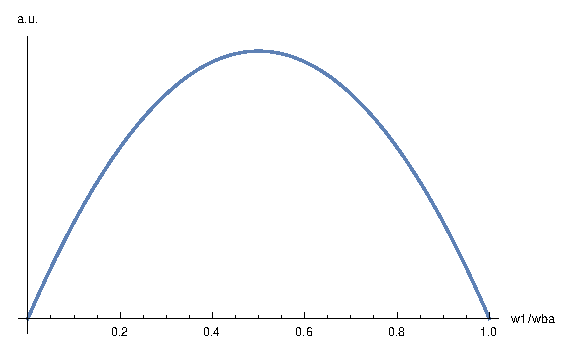
\includegraphics[width=0.5\textwidth]{aw1.eps}
		\end{figure}

	\end{enumerate}
\end{enumerate}
	
	
\end{document}








